\documentclass[sigconf,review=true]{acmart}

\begin{CCSXML}
	<ccs2012>
	   <concept>
		   <concept_id>10011007.10011006.10011072</concept_id>
		   <concept_desc>Software and its engineering~Software libraries and repositories</concept_desc>
		   <concept_significance>500</concept_significance>
		   </concept>
	 </ccs2012>
\end{CCSXML}
	
\ccsdesc[500]{Software and its engineering~Software libraries and repositories}
\keywords{data layout, data optimization, loop chains, inter-loop optimization, performance model}
\usepackage{array} 
\usepackage{comment}
\usepackage{graphicx}
\usepackage[T1]{fontenc}
\usepackage{csquotes}
\usepackage{balance}
\usepackage{setspace}

\usepackage{listings}
\usepackage{lstautogobble}
\usepackage{subcaption}

\usepackage{standalone}
\usepackage{algorithmicx}

\lstset{ %
language=C++,                % choose the language of the code
basicstyle=\ttfamily\footnotesize,       % the size of the fonts that are used for the code
commentstyle = \color{ForestGreen},
columns=fullflexible,
numbers=left,                   % where to put the line-numbers
numberstyle=\footnotesize,      % the size of the fonts that are used for the line-numbers
stepnumber=1,                   % the step between two line-numbers. If it is 1 each line will be numbered
numbersep=5pt,                  % how far the line-numbers are from the code
%backgroundcolor=\color{codeBG3},  % choose the background color. You must add \usepackage{color}
showspaces=false,               % show spaces adding particular underscores
showstringspaces=false,         % underline spaces within strings
showtabs=false,                 % show tabs within strings adding particular underscores
frame=single,           % adds a frame around the code
tabsize=2,          % sets default tabsize to 2 spaces
captionpos=b           % sets the caption-position to bottom
breaklines=true,        % sets automatic line breaking
breakatwhitespace=false,    % sets if automatic breaks should only happen at whitespace
keywordstyle=\color{blue},       % keyword style
  %language=Octave,                 % the language of the code
  otherkeywords={SearchVar,MV,TSS,tileExpr,Search,tFunc...},           % if you want to add more keywords to the set
  numberstyle=\tiny\color{black}, % the style that is used for the line-numbers
  rulecolor=\color{black},
escapeinside={<@}{@>}
} 
\definecolor{ForestGreen}{RGB}{34,139,34}
\newcommand{\todo}[1]{{\textcolor{red}{{\tt{TODO:}}\,\,#1 }}}
\newcommand{\nc}[0]{\todo{cite}}
\newcommand{\an}[1]{{\textcolor{blue}{Author's Note: #1}}}
\newcommand{\ttt}[1]{{\texttt{#1}}}
\usepackage{xspace}
\newcommand{\FormatDecisions}[0]{{\textsc{FormatDecisions}}}
\newcommand{\su}[1]{{#1$\times$}}
\graphicspath{{./graphics/}{.}}

\usepackage[subtle]{savetrees}
\vbadness=18000
\vfuzz=2pt
\title{\FormatDecisions{}: User-Guided Data Layout Optimization in RAJA}


% \author{Brandon Neth}
% \affiliation{%
% 	\institution{University of Arizona}
% 	\city{Tucson}
% 	\state{AZ}
% 	\country{USA}}
% \email{brandonneth@email.arizona.edu}

% \author{Thomas R.W. Scogland}
% \affiliation{
% 	\institution{Lawrence Livermore National Laboratory}
% 	\city{Livermore}
% 	\state{CA}
% 	\country{USA}}

% \author{Bronis R. de Supinski}
% \affiliation{
% 	\institution{Lawrence Livermore National Laboratory}
% 	\city{Livermore}
% 	\state{CA}
% 	\country{USA}}

% \author{Michelle Mills Strout}
% \affiliation{%
% 	\institution{University of Arizona}
% 	\city{Tucson}
% 	\state{AZ}
% 	\country{USA}}




\begin{document}



\begin{abstract}

The layout of data in memory is a key consideration in high performance computing applications.
From reducing cache and page misses to relieving pressure on memory bandwidth and avoiding inter-process communication, a good data layout improves performance at all levels of an application.
While performance portability libraries like RAJA and Kokkos incorporate the data's layout into its initialization, some applications benefit from changing the data layout between kernels.
Because these libraries do not support changing the data layout after initialization, application performance can suffer. 
We remedy this shortcoming by prototyping a lightweight, declarative API for changing data layouts between computations in RAJA.
We then extend the library with existing compiler technology to guide the use of layout changes based on our runtime performance model of their cost and benefit.
Thus, the model and runtime combine to \enquote{fill in} layout choices that the user did not specify.
Our approach provides the \FormatDecisions{} API that allows the user to specify as much of the layout information as they please and still obtain the performance benefits of changing data layouts.  
Further, because \FormatDecisions{} is built directly into the RAJA library, no additional build steps are required.
We evaluate \FormatDecisions{} on three benchmarks from the RAJAPerf Suite, where it achieves similar performance improvements to hand-implemented optimizations.
\end{abstract}
\maketitle
\def\@textbottom{\vskip \z@ \@plus 1pt}




\section{Introduction}
Data storage and access patterns are a key influence on overall application performance. 
For example, on a typical cache-based system, iterating through a two-dimensional array in column-order when data is stored in row-order can lead to significant slowdown. 
Although mechanisms such as compiler optimizations~\cite{wolf1991data,bixby1994automatic}
and data layout policies like those in Kokkos~\cite{edwards2014kokkos} and RAJA~\cite{hornung2014RAJA} can align data layout with computation schedules, compiler optimizations lack user controls and layout policies become difficult to automate and laborious to manage by hand as the number of loops and arrays grow.

Figure~\ref{IntroExample} shows the importance of a good data layout. 
The ``BadLayout" column shows the execution time for a matrix multiplication where the three arrays are laid out opposite of their access order. 
The ``GoodLayout" column shows the execution time for the same matrix multiplication when the arrays are laid out to match their access order.
The ``LayoutChange" column shows the execution time of code that changes the layout from the bad layout to the good one.
Finally, the ``SwitchAndRun" column shows the combined execution time of changing the layout from bad to good and then running.
As the graph shows, performance improves  significantly (72\%) simply by changing the data layout, and the cost of performing the layout change is small (<1\% of execution time). 

\begin{figure}
	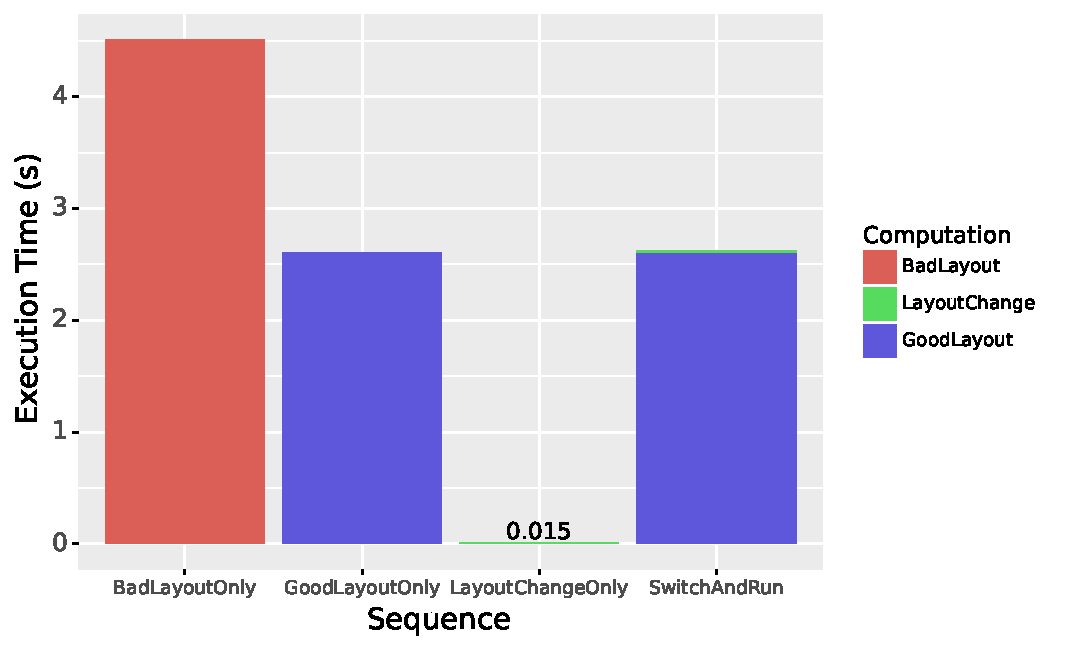
\includegraphics[width=\columnwidth]{IntroExampleGraph.pdf}
	\caption{Execution time for matrix multiplication using optimal and non-optimal data layouts and execution time for converting from non-optimal to optimal. Section~\ref{sec:systemDetails} for machine and compilation information.}
	\label{IntroExample}
	\Description[Matrix Multiplication Execution Time for Different Layouts]{A bar plot showing a "Bad Layout" column with execution time greater than the "Good Layout" and "Layout Conversion" columns combined.}
\end{figure}

General purpose libraries like Kokkos and RAJA and programming languages like Chapel~\cite{diaconescu2007approach} give programmers some control over the data layout of multi-dimensional arrays. However, this support is limited to the point of initialization.
Thus, programmers must use that particular data format for the entire computation.
While a developer could change the data layout mid-computation in RAJA, the developer must either modify RAJA library code or use multiple arrays for the same data. 
Both options increase the code complexity and increase its fragility.
The brave developer who chooses one of these options must still overcome yet another obstacle: selecting the right combination of formats.
Even a modest computation of two loops that use four 2D arrays has more than 200 combinations from which to choose, so trying all possible options quickly becomes infeasible. 

In this paper, we present \FormatDecisions{}, an approach for exposing data layout decisions to the programmer in the C++ portable, parallel library RAJA.
The presented API allows the programmer to specify as many data layout decisions in a sequence of data-sharing loops (otherwise known as a loop chain~\cite{krieger2013loop}) as they choose.
Then, using a portable cost model based on microbenchmarking, \FormatDecisions{} identifies any remaining layout changes estimated to improve performance. 

A significant body of work has developed Integer Linear Programming (ILP) formulations to determine data layouts in distributed memory settings for programming languages like HPF and D~\cite{bixby1994automatic,kennedy1995automatic,kennedy1998automatic}. 
A similar line of work~\cite{chen2004ilp,chen2005constraint,chen2005integrating, ozturk2011data} uses ILP-based constraint networks to combine data layout and schedule optimizations. 
Both approaches were developed in the context of a compiler. 
We build on their use of a performance model encoded as the objective function in an ILP problem to automate data layout decisions (partially or fully).
Rather than only applying this data layout technology in the compiler, we provide it to the user through a library interface while still enabling its automated use.
Our library and runtime approach allows the user to guide use of the technology to focus on loops most likely to benefit from it.
However, where a compiler can run complex analyses without a runtime cost, the library must perform its analysis and decision-making at runtime and the interface must be high-level while still providing enough control. 
While a library approach comes with runtime overhead, it is more accessible to users and has access to runtime information that the compiler may not, such as loop bounds.
Although useful advantages, these lead to sub-problems about how the library implementation can most leverage the compiler of the language in which it is embedded (C++ here) to force as much specialization as possible to achieve the ultimate goal of performance.

 


% We extend the RAJA C++ library to address this gap in support of data layout optimizations.
% First, \FormatDecisions{} exposes a lightweight API for implementing mid-computation data layout optimizations.
% We provide two methods --- \verb.set_format_before. and \verb.set_format_after. --- so the user can ensure the use of appropriate known formats \footnote{Since we completely expose the control, an autotuner can also try different options.}.
% While the user can specify any known formats, a performance model guides any unspecified choices.
% Based on run-time microbenchmarking, the model selects format changes through the solution of an ILP problem that considers the cost of converting formats against the potential improvement with an alternative format.
% Our inclusion of a performance model means a developer can obtain performance improvement without having to determine the sequence of format changes themselves.
% %% BRONIS: Most autotuning approaches do not use exhaustive testing
% %% BRONIS: I think one could argue that we use the ILP problem to autotune
% %% or use an autotuner to try every possible option.

This paper includes the following contributions:
\begin{itemize}
\item The \FormatDecisions{} API implemented in RAJA for specifying data layouts and data layout transformations;
\item A performance model to select data layouts based on runtime microbenchmarking and a data layout transformation strategy for a loop chain;
\item An optimization that increases the reuse of microbenchmarking information; and
\item Performance results and source lines of code (SLOC) for four variants of seven benchmark kernels comparing \FormatDecisions{} to hand-implemented optimization.
\end{itemize} 

The rest of the paper proceeds as follows. 
Section 2 reviews the RAJA library, prior extensions we use in the current work, and new support for symbolic description of iteration spaces.
Section 3 introduces the \FormatDecisions{} interface.
Sections 4 detail how we construct our performance model and estimate the costs of different layout conversion choices.
Sections 5 and 6 evaluate the impact of \FormatDecisions{}  on performance and productivity.
Section 7 reviews related work and section 8 concludes.


%%%%%%%%%%%%%%%
\section{Programming with RAJA}

\begin{figure}
	\begin{lstlisting}[
		caption={The \textsc{3mm} kernel (E = A * B, F = C * D, G = E * F) implemented using RAJA.},
		label={3MMStart}]
	// Array declarations with layout specifications
	auto row_major = make_permuted_layout(sizes, {{0,1}});
	auto column_major = make_permuted_layout(sizes, {{1,0}});

	View2D A(A_data, row_major);
	View2D B(B_data, column_major);
	... initializations proceed similarly for C-G with row_major

	// loop schedule
	using POLICY = KernelPolicy<
		statement::For<0,omp_parallel_for_exec,
			statement::For<1,loop_exec,
				statement::For<2,loop_exec,
					statement::Lambda<0>
				>
			>
		>
	>;

	// E = A * B;
	auto loop_body1 = [&](auto i0, auto i1, auto i2) {
		E(i0, i1) += A(i0,i2) * B(i2,i1);
	};
	// F = C * D;
	auto loop_body2 = [&](auto i0, auto i1, auto i2) {
		F(i0, i1) += C(i0,i2) * D(i2,i1);
	};
	// G = E * F
	auto loop_body3 = [&](auto i0, auto i1, auto i2) {
		G(i0, i1) += E(i0,i2) * F(i2,i1);
	};
	
	auto one_dim = RangeSegment(0,N);
	auto domain = make_tuple(one_dim, one_dim, one_dim);

	auto knl1 = make_kernel<POLICY>(domain, loop_body1);
	auto knl2 = make_kernel<POLICY>(domain, loop_body2);
	auto knl3 = make_kernel<POLICY>(domain, loop_body3);

	knl1();
	knl2();
	knl3();
	\end{lstlisting}
	\Description[RAJA Implementation of 3MM]{Fully described in the text.}
\end{figure}

\label{sec:kernelObjects}

We use a variety of components of the performance portability C++ library RAJA to enable automatic data format transformations, as well as features of the loop chain extension RAJALC~\cite{neth2021inter}. 
This section reviews how a computation is programmed in RAJA, the additions made by RAJALC, and how this work adds more expressive capabilities to the RAJA programming model.

\subsection{RAJA and RAJALC}

The foundational elements of RAJA are the execution constructs, \verb.forall. and \verb.kernel.. 
These templated functions execute a loop immediately, whereas the RAJALC \verb.make_forall. and \verb.make_kernel. extensions create wrapper objects that are executed through the call operator. 
Calls to \verb.make_kernel. can be seen in lines 40 through 42 in Listing~\ref{3MMStart}. 
While the RAJALC functions create computation objects rather than immediately executing the computation, their interfaces are the same as their base RAJA counterparts.

The execution constructs separate the specification of the computation from the specification of its schedule.
The template parameter describes the schedule of the computation as an execution policy, defined on lines 10 through 18.
Each level of the loop has its own schedule, where \verb.omp_parallel_for_exec. indicates an OpenMP parallel loop and \verb.loop_exec. indicates the compiler should make the decision.
Other policies exist for vectorization and GPU-offloading.
The runtime parameters describe the computation itself. 
The first parameter is the iteration space for the loop, in this case 3 dimensional, defined on lines 33 and 34. 
The second parameter is the loop body to execute for each iteration, passed as a lambda.
The three loop bodies are defined on lines 21 through 31.
After the computation objects are created on lines 36 through 38, they are executed through the call operator on lines 40 through 42.

RAJA also provides array wrappers called Views.
The View object has a number of capabilities that make it a valuable tool within RAJA codes.
First, Views use the call operator to perform memory accesses. 
By overloading this call operator for symbolic iterator types, RAJALC enables the runtime symbolic evaluation of kernels that use Views.
RAJALC uses the access information gathered from symbolic evaluation to ensure the correctness of its scheduling optimizations.
This work uses RAJALC's runtime symbolic evaluation to inform our performance model.
Second, Views fully parameterize their underlying data formats with the Layout object.
Without Views, to switch their data from row-major to column-major, a programmer must change the definition of the array \textit{and} must change every access \verb.A[i][j]. to \verb.A[j][i]..
This mechanism is prohibitively expensive, especially when the programmer does not yet know the performance impact of the decision.
With Views however, the programmer only needs to change the View's definition: the layout permutation changes from $(0,1)$ to $(1,0)$. 
In Listing~\ref{3MMStart}, \verb.A. is defined with the row-major $(0,1)$ layout, but \verb.B. is defined with the column-major $(1,0)$ layout. 
Note that the change in \verb.B.'s layout does not change how it is used in the computation. 

Throughout the computation, the data is accessed in different orders.
For example, consider the Views \verb.A., \verb.B., and \verb.D..
The order in which \verb.A. is accessed is different from \verb.D. because the argument order in their accesses are different.
In contrast, while \verb.B. and \verb.D. have the same argument order, their access orders are still different because they have different layouts.
Looking at the two references to \verb.F. in kernels two and three, we can see that even access order to the same data can change through a computation.
Because different formats are optimal for different kernels, this creates an opportunity for optimization. 


\subsection{Symbolic Iteration Spaces}
\label{sec:SymbolicSegment}
While RAJALC added support for kernel objects and the symbolic evaluation of those kernels, the description of a computation's iteration space was left unchanged. 
While RAJA can express a wide variety of computational patterns, it cannot express an important class of computations: those where inner loop bounds are a function of outer loop bounds.
A classic example of this pattern is the triangular iteration space, shown in Listing~\ref{TriangularIterationSpace}.
In such a loop nest, the bounds of the inner loop change with each iteration of the outer loop.
Standard RAJA has no way of cleanly expressing this relationship between the loop bounds, restricting the space of computations for which RAJA can be used.

We remedy this restriction by introducing a \verb.SymbolicSegment. type to the library. 
We also add a function for creating them, called \verb.make_symbolic_segment..
For segments with constant bounds, the \verb.SymbolicSegment. works the same as RAJA's other segment types. 
For example, line 8 of Listing~\ref{TriangularIterationSpace} shows how the outer loop bound from 0 to N is created.
For segments with bounds that are a function of outer loop values, the outer symbolic segment variable is used as a placeholder for its value during execution.
Line 9 shows how the inner loop bound is created as a function of the outer loop value.
While here we show a simple case, our approach supports all affine expressions of outer loop variables.
When it comes time to execute a kernel that uses symbolic segments, the values for inner loop bounds read the current value of the relevant outer loop iterator and use that to calculate the bounds for the nest.

\begin{figure}
	\begin{lstlisting}[caption={An example of a loop with a triangular iteration space, expressed in C++ and using our SymbolicSegments.},label={TriangularIterationSpace}]
// C++ implementation
for(int i = 0; i < N; i++) {
	for(int j = i; j < N; j++) {
		...
	}
}

auto i_seg = make_symbolic_segment(0,N);
auto j_seg = make_symbolic_segment(i_seg, N);
auto segs = make_tuple(i_seg, j_seg);

	\end{lstlisting}
	\Description[Triangular iteration space implemented in C++ and using our symbolic iteration space description.]{Fully described in the text.}
\end{figure}

\section{Transforming Data Layouts}

\begin{figure}
	\begin{lstlisting}[caption={Changing data layouts for one View in the \textsc{3mm} benchmark manually.},label={ByHand3MM}]
auto knl1 = make_kernel<KPOL>(segs1, [=](auto i0, auto i1, auto i2) {
	E(i0, i1) += A(i0, i2) * B(i2, i1);
});
auto knl2 = make_kernel<KPOL>(segs2, [=](auto i0, auto i1, auto i2) {
	F(i0, i1) += C(i0, i2) * D(i2, i1);
});
auto knl3 = make_kernel<KPOL>(segs3, [=](auto i0, auto i1, auto i2) {
	G(i0, i1) += E(i0, i2) * F(i2, i1);
});

knl1();

// Reorder F's data for row-major order
double * tmp1 = new double[n*n];
for(int i = 0; i < n; i++) {
	for(j = 0; j < n; j++){
		tmp1[i*n + j] = F(i,j);
	}
}
memcpy(F.data, tmp1, n*n);
F.layout = row_major;
delete[] tmp1;

knl2();

// Reorder F's data for column-major order
double * tmp2 = new double[n*n];
for(int i = 0; i < n; i++) {
	for(j = 0; j < n; j++){
		tmp2[j*n + i] = F(i,j);
	}
}
memcpy(F.data, tmp2, n*n);
F.layout = col_major;
delete[] tmp2;

knl3();
	\end{lstlisting}
	\Description[Manual implementation of layout transformation]{Fully described in the text.}
\end{figure}

\begin{figure}
\begin{lstlisting}[caption={Changing data layouts for three Views in the \textsc{3mm} benchmark using \FormatDecisions.},
	label={FormatDecisions3MM}]
auto knl1 = make_kernel<KPOL>(segs1, [=](auto i0, auto i1, auto i2) {
	E(i0, i1) += A(i0, i2) * B(i2, i1);
});
auto knl2 = make_kernel<KPOL>(segs2, [=](auto i0, auto i1, auto i2) {
	F(i0, i1) += C(i0, i2) * D(i2, i1);
});
auto knl3 = make_kernel<KPOL>(segs3, [=](auto i0, auto i1, auto i2) {
	G(i0, i1) += E(i0, i2) * F(i2, i1);
});

auto decisions = format_decisions(ref_tuple(B,D,F), knl1, knl2, knl3);

decisions.set_format_for(B, {{1,0}}, knl1); // column-major
decisions.set_format_for(D, {{1,0}}, knl2); // column-major
decisions.set_format_for(F, {{0,1}}, knl2); // row-major
decisions.set_format_for(F, {{1,0}}, knl3); // column-major

// Generate and run the computations with format conversions
auto computation = decisions.finalize();
computation();
\end{lstlisting}
\Description{Fully described in the text.}
\end{figure}

RAJA's existing support for changing data layouts is minimal. 
While Views can be instantiated with different layouts, changing the layout of an existing View is not as simple.
This is because changing layouts also requires reordering the underlying data to match the new layout. 
To implement such a layout change by hand requires the programmer to allocate a new temporary array, 
copy the data from the View to the temporary array in the right order, 
copy the data \textit{back} to the memory in the View, 
and then finally update the View's layout object.
This work removes that barrier by providing a declarative data optimization system and evaluating
it within the context of RAJALC.


\subsection{Declarative Layout Transformations}
Our approach, shown in action in Listing~\ref{FormatDecisions3MM}, introduces a single user-facing class, appropriately named \verb.FormatDecisions..
Rather than inserting code blocks to change a View's data layout between kernel executions, the user register choices for what format the data should have during different computations. Lines 13 through 17 of Listing~\ref{FormatDecisions3MM} show four such registered choices.
Once the user has finished registering their choices, \FormatDecisions{} looks for additional beneficial format conversions and generates a final computation object that makes format conversions and executes the computations, shown in lines 19 and 20.

\subsection{The \FormatDecisions{} API}
The \FormatDecisions objects are initialized using the \\
 \verb.format_decisions. function with the data to potentially transform and the computations in which the data is used.
\FormatDecisions{} supports four operations: registering format decisions, turning the supplementary modeling on and off, running the supplementary model, and generating the final computation.

The user registers format decisions with two methods.
The first, \verb.set_format_for()., takes as arguments the View, the desired dimensional ordering, and the computation.
Without requiring that the conversion occurs immediately before the computation, it ensures that while that computation executes the View has the desired format.
The second method, \verb.set_output_format()., takes a View and a dimensional ordering and ensures the View has that layout after the sequence of computations is done executing.


While we provide a supplementary decision model that can identify additional worthwhile layout changes, its use is not mandatory.
In the case where the user does not want the supplementary model to run, they can use the \verb.lock(). method. 

Regardless of whether the user has turned the model off or left it on, 
after the user has registered their choices, the complete computation with interspersed format conversions is generated using the \verb.finalize. method.
If the user does not call the \verb.lock. method, this function also runs the model to identify additional changes that may be beneficial. The model does not overwrite user-registered decisions.

\subsection{Selecting Decision Semantics}

At first glance, it may seem that a single method for registering format choices would be sufficient. 
Simply provide the View, the computation, and the format to use during that computation.
However, it is often desirable to specify the format the data should be in at the end of the sequence of computations, especially when the sequence is run many times, for example as part of the time step in a simulation code.
A single registering function cannot provide this capability. 

Another important consideration is the semantics of the registered decisions. 
Should the user be registering format conversions or should they be registering the format with the assumption that any necessary conversion is made by the library?
We argue that it should be the latter.
First, registering formats is more declarative, as it does not dictate exactly how or when the data is converted to the desired format.
Second, registering conversions requires specification of both the input and output formats. 
Any conversion can be specified with two format registrations, but no number of conversion registrations can specify the same thing as a single format registration.

With these considerations in mind, we decided on two methods: \verb.set_format_for. and \verb.set_output_format..
When choosing this pair, the shorter \verb.set_format. was considered, but lacks the mneumonic match between the words of the method name and the order of the parameters. We \textbf{set} the View to \textbf{format} X \textbf{for} computation Y. 



%%%%%%%%%%%%%%%%%%%%%%%%%
\section{Constraint Model for Supplementary Transformations}

In addition to the format changes registered by the user, \FormatDecisions{} also uses a constraint model to determine if additional format changes would improve performance. 
This capability means that even without any registered format choices, \FormatDecisions{} often selects the same changes the user would themselves choose.
We encode the problem as an optimization problem where constraints encode registered decisions and the objective function encodes the estimated costs of format use and conversion.

This optimization problem can intuitively formulated as a graph problem in which nodes represent using a format for a computation and the edges represent conversions between formats~\cite{kennedy1998automatic}.
Then, nodes and edges are assigned weights based on the cost of using that format or making that conversion. 
In this formulation, the shortest path through the graph represents the optimal set of formats and conversions to use.

\subsection{Constraining the Decision Space}
Figure~\ref{graphModel} shows the constraints used to model the View \verb.F. from Listing~\ref{FormatDecisions3MM}.
The variables of this optimization problem are boolean decision variables representing the possible format choices. 
For this example, there are 10 total decision variables: 2 for the input formats, 2 for each computation, and 2 for the output formats.

At the beginning, the only imposed constraint is that a View can only have one format at a time, indicated by the red, undirected edges among the nodes in Figure~\ref{graphModel:1}.
Algebraically, this means that the sum of the variables for a specific computation must sum to 1. 

As decisions are registered, constraints are added that set the appropriate decision variables to 1, indicated by the green, outlined nodes in Figures~\ref{graphModel:2} and \ref{graphModel:3}. 
Because of the single-format constraints, we also know that the other decision variables for those computations must be set to 0, indicated by dark grey nodes.

When it comes time to solve the model, the input format variables are set based on the actual format of the data at solve time. This is shown with the green, outlined rhombus node in Figure~\ref{graphModel:4}.




\begin{figure}
	\begin{subfigure}[t]{0.2\textwidth}
		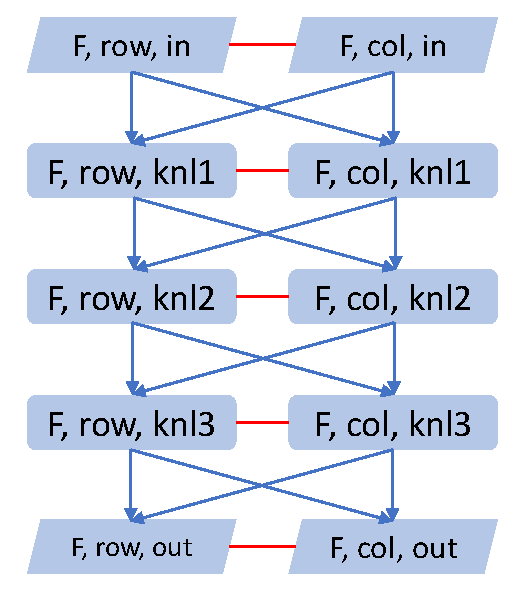
\includegraphics[page=1,width=\textwidth]{ModelProgression.pdf}
		\caption{Initial state of the optimization problem.}
		\label{graphModel:1}
	\end{subfigure}
	\hspace{0.05\textwidth}
	\begin{subfigure}[t]{0.2\textwidth}
		\includegraphics[page=2,width=\textwidth]{ModelProgression.pdf}
		\caption{After registering that F should be row-major during the second computation.}
		\label{graphModel:2}
	\end{subfigure}

	\begin{subfigure}[t]{0.2\textwidth}
		\includegraphics[page=3,width=\textwidth]{ModelProgression.pdf}
		\caption{After registering that F should be column-major during the third computation.}
		\label{graphModel:3}
	\end{subfigure}
	\hspace{0.05\textwidth}
	\begin{subfigure}[t]{0.2\textwidth}
		\includegraphics[page=4,width=\textwidth]{ModelProgression.pdf}
		\caption{After the input format has been set and before the problem is solved. The model picks the output format and the format for knl1.}
		\label{graphModel:4}
	\end{subfigure}

	\vspace{5px}

	\begin{subfigure}{0.45\textwidth}
		\begin{align*}
			x_{(F,row,in)} + x_{(F,col,in)} = 1 &\wedge 
		x_{(F,row,knl1)} + x_{(F,col,knl1)} = 1 \wedge \\
		x_{(F,row,knl2)} + x_{(F,col,knl2)} = 1 &\wedge 
		x_{(F,row,knl3)} + x_{(F,col,knl3)} = 1 \wedge \\
		x_{(F,row,out)} + x_{(F,col,out)} = 1 &\wedge 
		x_{(F,row,knl2)} = 1 \wedge\\
		 x_{(F,col,knl3)} = 1 &\wedge x_{(F,row,in)} = 1
		\end{align*}
		
		\caption{The algebraic representation of the constraints present when the problem is solved.}
		\label{graphModel:5}
	\end{subfigure}

	\caption{Graphical representation of the layout optimization problem for a View in \textsc{3mm}. Nodes represent possible format choices and edges represent format conversions. User choices constrain the possible paths through the graph.}
	\label{graphModel}
	\Description[Optimization Graph Constraints]{Four directed graphs with edges progressively removed.}
\end{figure}

\subsection{Constructing the Objective Function}

The objective function for our model estimates the runtime performance of different format choices by considering the costs of format uses and format conversions.

Each View reference in the computation contributes one term to the objective function for each possible data layout. This means that the reference \verb.F(i2,i1). in \verb.knl3.  contributes two terms.
The first term,  $c * x_{(F,row,knl3)}$,  represents the cost of that reference if \verb.F. were in row-major order. 
The second term, $c^\prime * x_{(F,col,knl3)}$  represents the cost of that reference if \verb.F. were in column-major order.
Because \verb.F. is not referenced in the first kernel, the objective function does not contain linear terms for either $x_{(F,row,knl1)}$ or $x_{(F,col,knl1)}$.
However, these decision variables appear in terms for format conversion costs.

Because a format conversion depends the format coming in and going out of the conversion, jconversion cost terms contain two decision variables.
For example, consider the conversion step between \verb.knl1. and \verb.knl2..
There are two possible conversions to consider: row-major to row-major and column-major to row-major. 
Converting from row-major to row-major requires no action, so we  find the term $0 * x_{(F,row,knl1)} * x_{(F,row,knl2)}$ in the objective function.
Converting from column-major to row-major does require a reformating, so we  also find a term $c^{\prime\prime} * x_{(F,col,knl1)} * x_{(F,row,knl2)}$ in the objective function.

Once the objective function is constructed, we can search for the format choices that minimize it, but first we need to determine the actual values for the cost coefficients.

\subsection{Determining Cost Coefficients}

Accurate estimations are key to selecting formats with good performance, so we use runtime microbenchmarking to incorporate empirical, system-specific profiling data into the model.
However, because this microbenchmarking occurs at runtime, the overhead can meaningfully impact overall performance. 
To mitigate this effect, we reuse microbenchmarking results by modeling choices based on their access order.
The access order for a View reference encodes the ordering of the index arguments, the View's layout, and the kernel's execution policy.
By normalizing the policy and layout orders, we can map accesses to a much smaller set of values to estimate.
This subsection explains how we calculate access orders and argues that the access order is an accurate predictive metric for the relative performance of a layout choice. 

\begin{figure*}

	\begin{subfigure}{0.9\textwidth}
		\begin{center}
			\begin{tabular} {|c|c|c|}
				\hline
				Kernel & Policy Order \\ \hline 
				knl1 & (0,1,2) \\
				knl2 & (2,0,1) \\
				\hline
			\end{tabular}
			\hspace{0.01\textwidth}
			\begin{tabular} {|c|c|c|}
				\hline 
				View & Argument Order & Layout Order \\  \hline 
				A & (0,2) & (0,1) \\ 
				B & (2,1) & (1,0) \\
				C & (0,1) & (0,1) \\
				\hline
			\end{tabular}
			\hspace{0.01\textwidth}
			\begin{tabular} {|c|c|c|}
				\hline
				Information & Source \\ \hline 
				Argument Order & Symbolic evaluation  \\
				Layout Order & Symbolic evaluation \\
				Policy Order & Template parameter \\
				\hline
			\end{tabular}
		\end{center}
		\caption{The information used to calculate access orders and how they are collected. Policy orders come from the policies on lines 12-30, argument orders from the View references on line 9, and layout orders from the data initialization on lines 1-6.}
		\label{accessOrder:orders}
	\end{subfigure}

	\vspace{10px}

	\begin{subfigure}[b]{0.40\textwidth}
		\begin{lstlisting}
auto row_major = make_permuted_layout(sizes, {{0,1}});
auto column_major = make_permuted_layout(sizes, {{1,0}});

View2D A(a_data, row_major); 
View2D B(b_data, column_major); 
View2D C(c_data, row_major);

auto matmul_lambda = [&](auto i0, auto i1, auto i2) {
	C(i0,i1) += A(i0,i2) * B(i2,i1);
}

using Policy_012 = KernelPolicy< 
	statement::For<0,loop_exec, // for i
		statement::For<1,loop_exec, // for j
			statement::For<2,loop_exec, // for k
				statement::Lambda<0>
			>
		>
	>
>;

using Policy_201 = KernelPolicy< 
	statement::For<2,loop_exec, // for k
		statement::For<0,loop_exec, // for i
			statement::For<1,loop_exec, // for j
				statement::Lambda<0>
			>
		>
	>
>;

auto knl1 = make_kernel<Policy_012>(domain, matmul_lambda);
auto knl2 = make_kernel<Policy_201>(domain, matmul_lambda);
		\end{lstlisting}
		\caption{Two kernels implementing matrix multiplication using different execution policies. The change in policy is equivalent to exchanging the loop nest order.}
		\label{accessOrder:code}
	\end{subfigure}
	\hspace{0.02\textwidth}
	\begin{subfigure}[b]{0.45\textwidth}
		\begin{center}
		Argument Order $\xrightarrow[\text{Layout Order}]{permute}$ Layout-Normalized Order

		Layout-Normalized Order $\xrightarrow[\text{Policy Order}]{indexof}$ Access Order

		\vspace{5px}
		\dots\dots\dots
		\vspace{5px}

		knl1, A: $(0,2)$ $\xrightarrow[(0,1)]{permute}$ $(2,0)$ $\xrightarrow[(0,1,2)]{indexof}$ $(2,0)$.
		
		knl1, B: $(2,1)$ $\xrightarrow[(1,0)]{permute}$ $(1,2)$ $\xrightarrow[(0,1,2)]{indexof}$ $(1,2)$.
		
		knl1, C: $(0,1)$ $\xrightarrow[(0,1)]{permute}$ $(0,1)$ $\xrightarrow[(0,1,2)]{indexof}$ $(0,1)$.
		
		knl2, A: $(0,2)$ $\xrightarrow[(0,1)]{permute}$ $(2,0)$ $\xrightarrow[(2,0,1)]{indexof}$ $(0,1)$.

		knl2, B: $(2,1)$ $\xrightarrow[(1,0)]{permute}$ $(1,2)$ $\xrightarrow[(2,0,1)]{indexof}$ $(2,0)$.

		knl2, C: $(0,1)$ $\xrightarrow[(0,1)]{permute}$ $(0,1)$ $\xrightarrow[(2,0,1)]{indexof}$ $(1,2)$.
	\end{center}
	\caption{The calculation process. The first transformation normalizes different layouts. The second normalizes different policy orders. The resulting tuple represents the canonical data access with the same performance behavior. References with the same access order can be modeled with the same microbenchmark.}
	\label{accessOrder:calc}
	\end{subfigure}

	
	\caption{Calculating access orders for the View references in two matrix multiplication kernels. \ref{accessOrder:orders} shows the information extracted from \ref{accessOrder:code}. \ref{accessOrder:calc} shows how this information is used to estimate multiple reference costs with the same microbenchmark. }
	\label{accessOrder}
	\Description[Access Order Extraction]{Three panels. The first shows two implementations of matrix multiplication, the second the calculation process for extracting access orders, and the third the information extracted from the kernel that is used to generate the access order.}
\end{figure*}


Figure~\ref{accessOrder} details the process of calculating access orders. 
In Figure~\ref{accessOrder:code}, we see the implementation of two slightly different matrix multiplication kernels. 
While the data and loop body lambda are identical, they differ in their kernel policy, which determine how the kernel traverses the iteration space.
The kernel policy orders are shown in Figure~\ref{accessOrder:orders}, alongside the order of each View's indexing arguments and layout.
The policy orders are part of the type of the kernel, while the argument and layout orders of the Views are gathered from the symbolic evaluation of the kernel lambdas.
Figure~\ref{accessOrder:calc} presents the general approach and examples of calculating the access order.
Starting with the argument index order, we permute by the layout order then map values to their indices in the policy order.

Our claim is that the access order of an View reference is an accurate predictive metric for the relative performance of a layout choice.
We support this claim empirically using performance data from three microbenchmarks.
For each microbenchmark, we record the 5-run average execution time of all combinations of policy, layout, and argument order. 
These execution times are then grouped by access order.

If our claim is valid, then the execution times for each access order will cluster and the groups of execution times will not overlap.
Microbenchmark 1 is an access to a 3-dimensional View in a 3-dimensional loop, and is representative of the microbenchmark used to estimate costs within \FormatDecisions. 
Microbenchmark 2 is an access to a 2-dimensional View in a 3-dimensional loop, as in a matrix multiplication.
Microbenchmark 3 is an access to a 3-dimensional View in a 4-dimensional loop for a set argument order.
Table~\ref{MicrobenchmarkDetails} summarizes them in more detail, including data sizes.
The outermost loop is parallelized using OpenMP.
See Section~\ref{sec:systemDetails} for machine and compilation information.
\label{sec:AccessMetric}
\begin{table}
	\centering
	\begin{tabular}{|p{2.2cm}|p{1.6cm}|p{1.6cm}|p{1.5cm}|}
		\hline
		\raggedright Microbenchmark \linebreak Number & \raggedright \# View \linebreak Dimensions & \raggedright \# Loop \linebreak Dimensions & \raggedright Size per \linebreak Dimension \tabularnewline
		\hline
		1 & 3 & 3 & 128 \\
		2 & 2 & 3 & 512 \\
		3 & 3 & 4 & 64 \\
		\hline
	\end{tabular}
	\caption{Microbenchmark details for evaluating access order as a performance metric.}
	\label{MicrobenchmarkDetails}
\end{table}

\begin{figure*}
  \centering
  \begin{subfigure}{0.48\textwidth}
	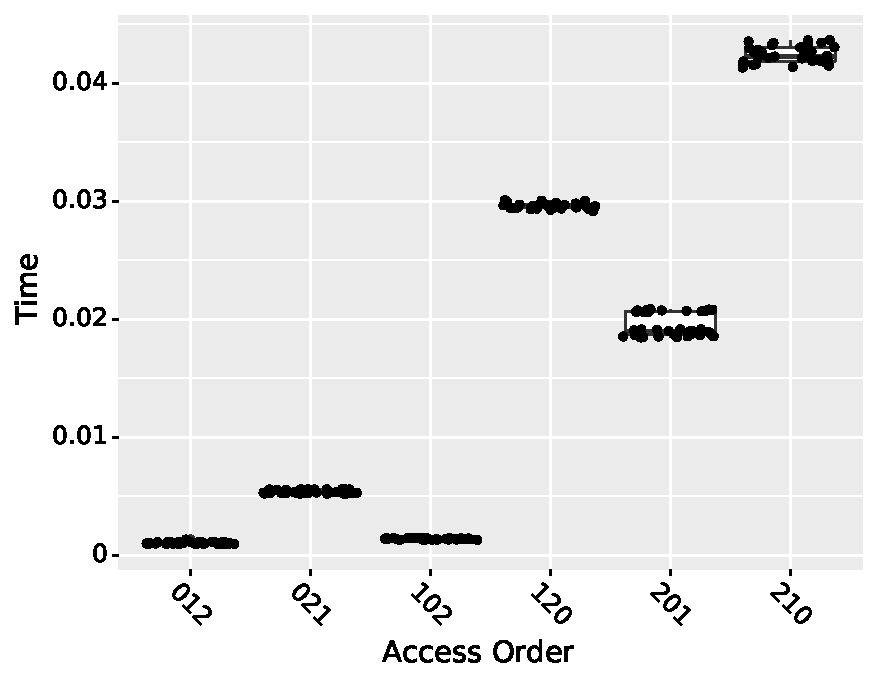
\includegraphics[width=\textwidth]{benchmark1_boxplot.pdf}
	\caption{Box plots showing execution times for a 3-dimensional loop accessing a 3-dimensional View, grouped by access order. }
	\label{AccessBenchmark1}
	\Description[Access Order Execution Times Boxplot for Microbenchmark 1]{Fully described in the text.}
  \end{subfigure}
  \hfill
\begin{subfigure}{0.48\textwidth}
	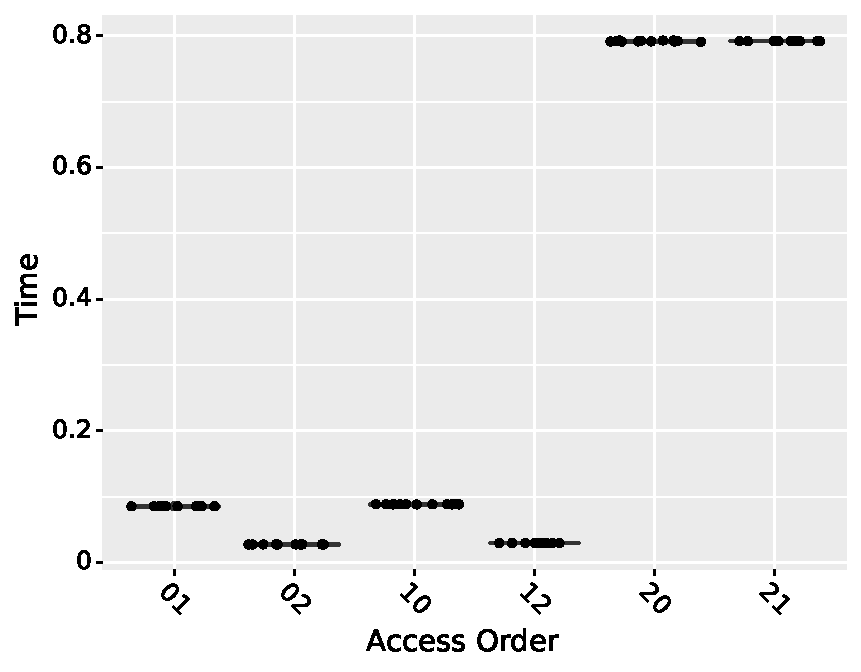
\includegraphics[width=\textwidth]{benchmark2_boxplot.pdf}
	\caption{Box plots showing execution times for a 3-dimensional loop accessing 2-dimensional View, grouped by access order. }
	\label{AccessBenchmark2}
	\Description[Access Order Execution Time Boxplot for Microbenchmark 2]{Fully described in the text}
\end{subfigure}

\bigskip
\begin{subfigure}{0.48\textwidth}
	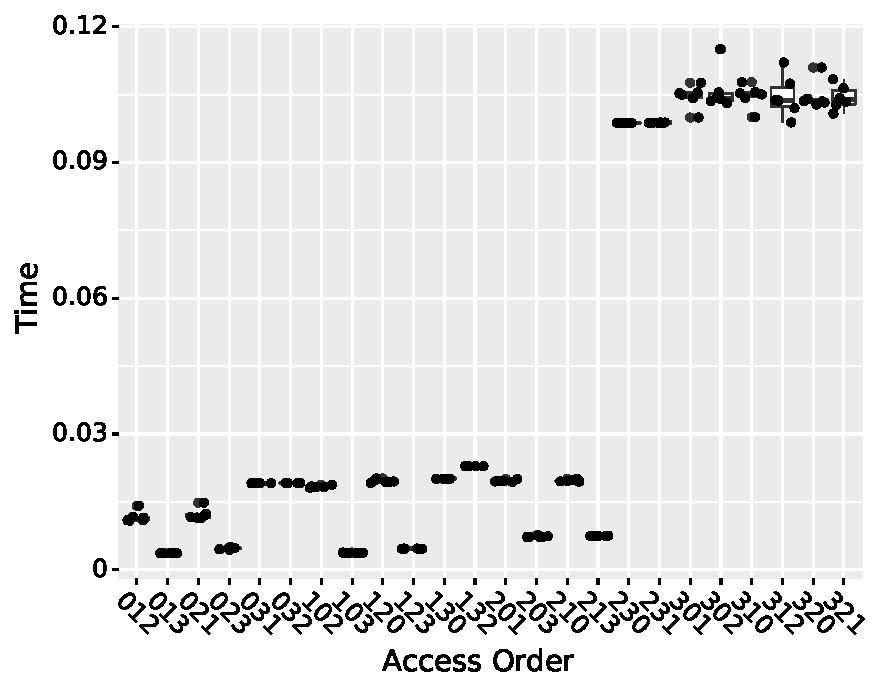
\includegraphics[width=\textwidth]{benchmark3_boxplot.pdf}
	\caption{Box plots showing execution times for a 4-dimensional loop accessing a 3-dimensional View, grouped by access order.}
	\label{AccessBenchmark3}
	\Description[Access Order Execution Time Boxplot for Microbenchmark 3]{Fully described in the text}
\end{subfigure}

\caption{Execution times for three microbenchmarks using different access orders. Each access order group is jittered.}
\end{figure*}

Figure~\ref{AccessBenchmark1} shows the execution times for the different access orders for microbenchmark 1.
Overall, the six possible access orders show good differentiation and clustering.
The access order $(2,0,1)$ does show two subclusters, but remain highly distinct from the other access order groupings. 
Additionally, access orders $(0,1,2)$ and $(1,0,2)$ show some overlap, likely because the bulk of the performance improvement comes from the innermost loop in a nest traversing the stride-one dimension of the data.
We also hypothesize that the different between orders $(0,2,1)$ and $(2,0,1)$ is due to better data partitioning for the threads in the $(0,2,1)$ order. 
Figure~\ref{AccessBenchmark2} shows the execution times for the different access orders for microbenchmark 2. 
This microbenchmark also shows good cluster and differentiation.
Like microbenchmark 1, the access orders $(0,2)$ and $(1,2)$ have similar performance, likely for the same reason. 
Figure~\ref{AccessBenchmark3} shows the execution times for the different access orders for microbenchmark 3.
A similar pattern as the previous microbenchmarks emerges here: grouping based on the position of the innermost iterator. 


%%%%%%%%%%%%%%%%%%%%%%
\section{Experiment 1: RAJAPerf and miniQMC}
\label{sec:Experiment1}

Our first evaluation experiment examines application performance and programmer productivity using seven benchmarks.
Six come from the Polybench~\cite{pouchet2012polybench} section of the RAJAPerf suite~\cite{hornung2017raja}. 
Of those six, we added four--\textsc{correlation}, \textsc{covariance}, \textsc{doitgen}, and \textsc{symm}--for this contribution. 
The seventh kernel, \textsc{qmc}, is based on the determinant update from the miniQMC miniapp~\cite{richards2018fy18}.




\textsc{2mm} solves the matrix expression $A*B*C$ using two matrix multiplications. 
First, it computes $A*B$ and stores the results in a temporary array.
Then this temporary result is multiplied by $C$.
\textsc{3mm} solves a similar matrix expression $A*B*C*D$ using three matrix multiplications.
It computes $A*B$, then $C*D$, then multiplies the results.
\textsc{correlation} and \textsc{covariance}, as the names suggest, calculate the correlation and covariance matrix for the input data. 
\textsc{correlation} has four loop nests and \textsc{covariance} has three.
\textsc{doitgen} is a multiresolution analysis kernel while \textsc{symm} computes a symmetric matrix-multiplication.
\textsc{qmc} uses three matrix multiplications to update an inverted matrix. 

\begin{table}
	\centering
	\begin{tabular}{| p{2.4cm} | p{1.1cm} | p{1.1cm} | p{1cm} | p{1cm}|}
		\hline
		 \raggedright Variant \linebreak Name & \raggedright Kernel Objects & \raggedright Layout Changes & \raggedright Chosen By &  Written Using \tabularnewline
		\hline
		\verb.RAJALC. & Yes & No & - & - \\
		\verb.Hand_Layout. & Yes & Yes & User & No API \\
		\verb.Format_Decision. & Yes & Yes & User & API \\
		\verb.Model_Choice. & Yes & Yes & Model & API \\
		\hline
	\end{tabular}
	\caption{Benchmark variant descriptions.}
	\label{VariantDescription}
\end{table}
For each benchmark, we implement 4 variants and compare execution time and code length, shown in Table~\ref{VariantDescription}.
\verb.RAJALC. implements the computations using the kernel objects discussed is Section~\ref{sec:kernelObjects}. 
\verb.Hand_Layout. implements identified transformations without using \FormatDecisions. 
Because this variant does not have any analysis overhead, we expect this variant to be the fastest.
The \verb.Format_Decision. variant uses \FormatDecisions to register the identified layout changes but does not use the model to look for other beneficial transformations.
Last, \verb.Model_Choice. allows the decision model to make all layout choices without providing any user-identified transformations.

\subsection{Performance Evaluation}
All performance results in this paper were collected on a single node with a 44-core IBM Power9 CPU and 256GB of CPU memory. 
We run with 22 threads on one socket to avoid transfers over a relatively slow inter-socket connection.
All compilation used GCC version 8.3.1 with \verb.-O3. optimization.
\label{sec:systemDetails}
Figure~\ref{fig:speedups} reports the average speedup of the variants relative to the \verb.RAJALC. variant across 5 runs. 

\begin{figure*}
	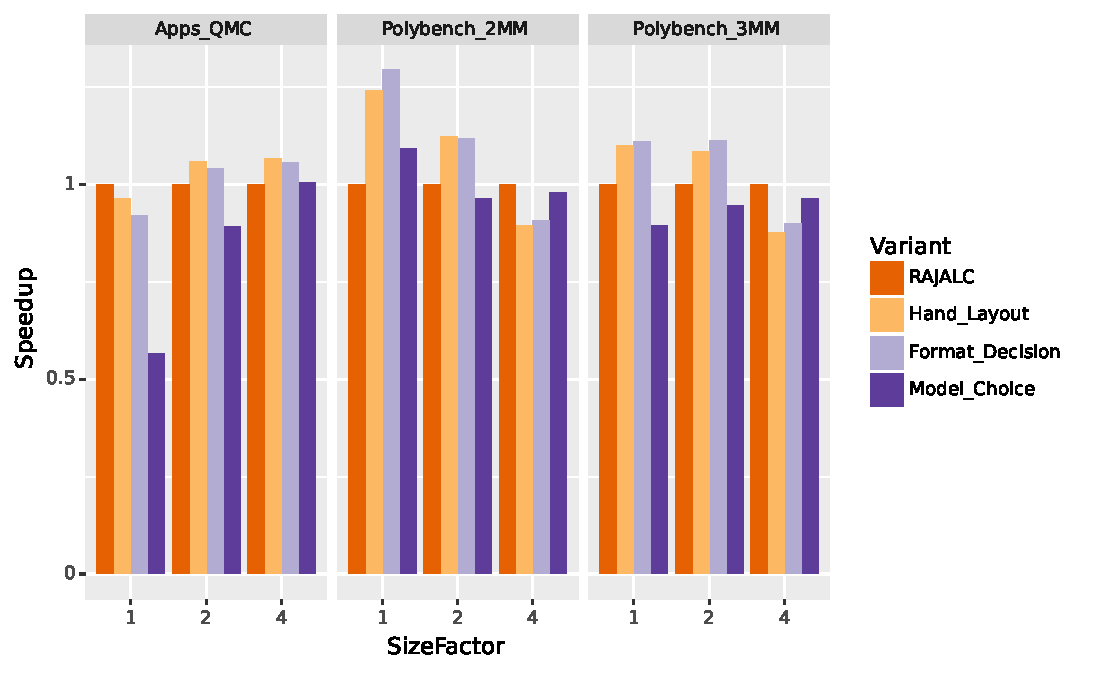
\includegraphics[width=0.9\textwidth]{speedups.pdf}
	\caption{Relative speedups of the different variants for different problem size factors. Speedup is calculated in reference to the RAJALC variant. Higher is better.}
	\label{fig:speedups}
	\Description[Polybench Speedups]{Bar chart for the speedup of the different Polybench kernels. Each kernel has a cluster of four bars, one for each variant. }
\end{figure*}

For the \textsc{2mm} and \textsc{3mm} kernels, the performance of the three layout-changing variants are comparable. 
For the standard (SizeFactor=1) problem size, the performance effects are minimal, with \verb.Hand_Layout. providing a 1.003$\times$ and 1.006$\times$ speedup to \textsc{2mm} and \textsc{3mm} respectively. 
The \verb.Format_Decision. variant provides a small 1.002$\times$ speedup to \textsc{2mm} and 1.003$\times$ to \textsc{3mm}, while the \verb.Model_Choice. variant shows a decrease in performance of 0.997$\times$ and 0.987$\times$, respectively. 
For the middle problem size (SizeFactor=2), the performance effects of layout transformations are greater. 
For \textsc{2mm}, we see a 1.111$\times$ speedup for the \verb.Hand_Layout. variant and 1.110$\times$ speedups for \verb.Format_Decision. and \verb.Model_Choice. 
For \textsc{3mm}, we see a similar pattern slightly modified by the higher modeling costs of the \textsc{3mm} kernel. \verb.Hand_Layout. gives a 1.083$\times$ speedup, \verb.Format_Decision. a 1.081$\times$ speedup, and \verb.Model_Choice. a 1.076$\times$ speedup.
For the large problem size (SizeFactor=4), the results are similar.
All three variants of \textsc{2mm} see a 1.084$\times$ speedup, whereas the variants of \textsc{3mm} see a 1.080$\times$, 1.079$\times$, and 1.078$\times$ speedup.

For \textsc{correlation}, there is less variability across problem sizes. 
For SizeFactors 1, 2, and 4, the \verb.Hand_Layout. variant sees speedups of 1.046$\times$, 1.076$\times$, and 1.086$\times$, respectively. 
The \verb.Format_Decision. variant does slightly better with speedups of 1.052$\times$, 1.086$\times$, and 1.096$\times$.
\verb.Model_Choice. remains competitive at 1.049$\times$, 1.086$\times$, and 1.087$\times$.
The \textsc{covariance} kernel performs similarly.

The \textsc{doitgen} kernel sees relatively flat performance across problem sizes and variants. All speedups are within 1\% of the baseline except \verb.Hand_Layout. at SizeFactor=2, with a speedup of 1.011$\times$. 

\textsc{qmc} fairs similarly to \textsc{doitgen}, although it sees more significant slowdowns. 
At the standard problem size, \verb.Hand_Layout. and \verb.Format_Decision. see small slowdowns of 0.995$\times$ and 0.982$\times$. 
The \verb.Model_Choice. has a more significant slowdown at 0.891$\times$ due to the overhead costs of running the model.
For the larger problem sizes, this cost has less influence, at 0.971$\times$ at SizeFactor=2 and 0.995$\times$ at SizeFactor=4. 

The \textsc{symm} kernel performs less consistently than the other kernels, but still sees directional matching between the \verb.Hand_Layout. and \verb.Format_Decision. variants.
The standard problem size gives a 1.018$\times$ speedup for \verb.Hand_Layout., a more significant 1.135$\times$ for \verb.Format_Decision., and a slowdown of 0.867$\times$ for \verb.Model_Choice.. 
We attribute this slowdown for the standard problem size to the smaller amount of computation in the \textsc{symm} kernel that can offset the cost of the performance modeling. 
For SizeFactor=2, we see speedups across the board, at 1.032$\times$, 1.174$\times$, and 1.053$\times$ respectively.
Finally, for SizeFactor=4, \verb.Hand_Layout. and \verb.Format_Decision. give speedups of 1.046$\times$ and 1.175$\times$ while \verb.Model_Choice. gives a speedup of 1.075$\times$.


\subsection{Productivity Evaluation}

To evaluate the productivity of \FormatDecisions{}, we report the source lines of code added or changed for each of the variants.
This value is calculated by counting the number of line differences using python's \verb.Differ.. 
We preprocess to remove all whitespace-only lines.
Figure~\ref{PolybenchSLOC} shows the results.
With the exception of \textsc{3mm} and \textsc{qmc}, using \FormatDecisions{} requires between 2 and 3$\times$ fewer code changes than implementing the transformations by hand. 
When using the performance model to make the layout choices, this is reduced further, requiring 4 to 6$\times$ fewer code changes. 

While the productivity benefit here is significant, \FormatDecisions{} is especially useful when making subsequent layout changes after the first. 
Once a code has been changed to use \FormatDecisions{}, the change quantified in Figure~\ref{PolybenchSLOC}, further changes can be introduced with only a single line. 
For example, manually tuning data layouts for a new machine amounts to a handful of reordered characters to describe the new layouts. 

Perhaps more important than the simple number of code changes when trying out new layouts is the ease of mistakes when implementing those transformations by hand. 
When using \FormatDecisions{}, all the complexity of ensuring the transformations go as planned is boiled down to one method call.
In the hand-implemented case, the programmer is responsible for correctly declaring the new data layout, optimizing the transformation itself, and appropriately updating the data structure to the new layout, among other things. 
Forgetting one of these steps, or mistyping the desired data layout, can lead to incorrect results that could be caused by any of the different components.
By removing this complexity, \FormatDecisions{} reduces the mental load on the programmer, freeing up capacity to explore more possible implementations.
Overall, \FormatDecisions{} provides comparable--and sometimes better--performance improvements without the code complexity of implementing the transformations by hand.



\begin{figure}
	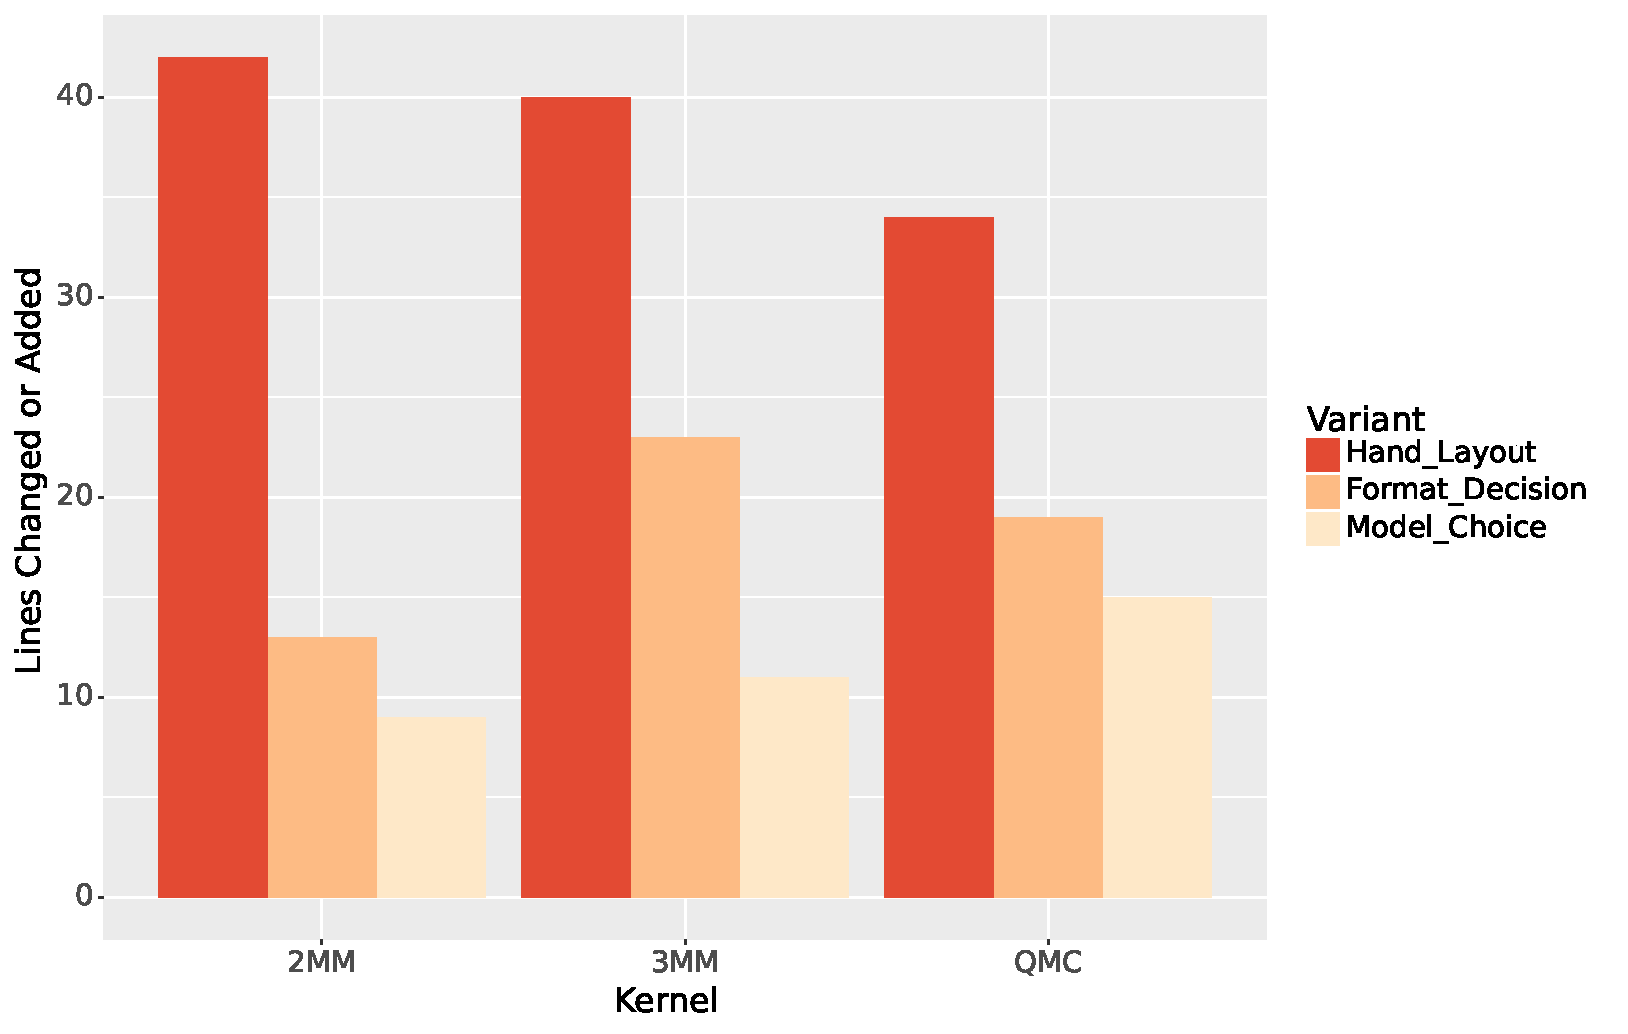
\includegraphics[width=\columnwidth]{sloc.pdf}
	\caption{Source lines of code modified (added, changed, or removed) relative to the  RAJALC variant. (Lower is better)}
	\label{PolybenchSLOC}  
	\Description[Polybench SLOC]{Bar chart for the source lines of code changed for the different Polybench kernels. Each kernel has a cluster of four bars, one for each variant that is not the baseline.}
\end{figure}


\section{Experiment 2:  Exhaustive Search for \textsc{2mm}}

Our second experiment further examines the efficacy of our model. 
Whereas the experiments of in Section~\ref{sec:AccessMetric} examined the efficacy of access order representing individual accesses, this experiment considers the model as a whole.
For the \textsc{2mm} benchmark, we evaluated the performance of all possible format choices and compare their execution times against their model scores (the value of the objective function for that choice).
We average execution times over five runs.
The absolute accuracy of our model is measured by the correlation between the execution time and the model score.
However, we are most interested in the \textit{relative} accuracy of our model.
A model is more relatively accurate when choices with better model scores have lower execution times, regardless of the specific values of the score or execution time.

\begin{figure}
	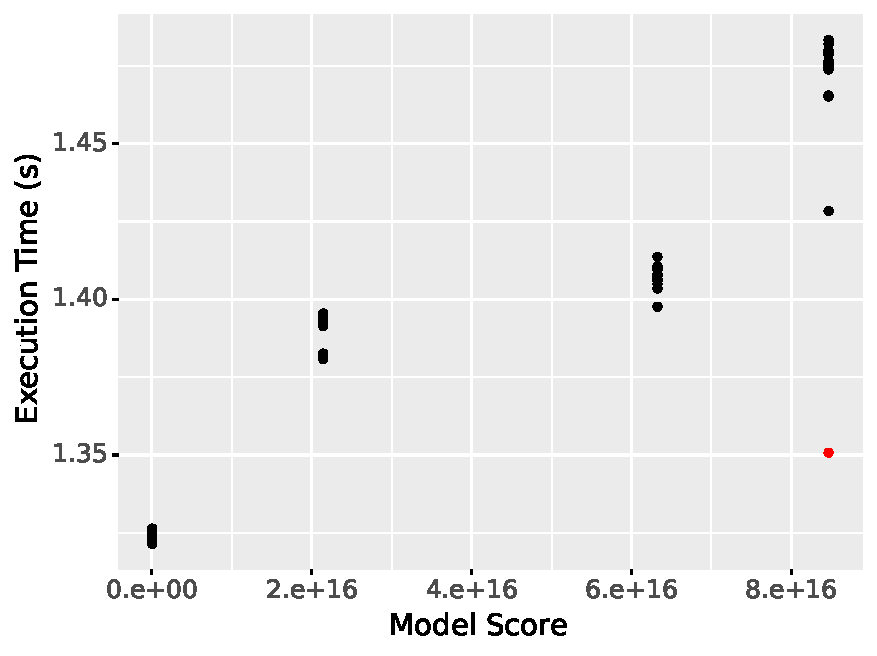
\includegraphics[width=\columnwidth]{2mm-all.pdf}
	\caption{Execution time and model score of all possible format choices for the \textsc{2mm} kernel. The model selects the choice with the lowest score. Outlier shown as red triangle. All dimension sizes are 1024.}
	\label{2MMAllChoices}
	\Description[Model Score and Execution Time]{Fully described in the text.}
\end{figure}


Figure~\ref{2MMAllChoices} plots the model scores and execution times for the different choices. 
While the overall relationship between model score and execution is as expected, there is one notable outlier, colored in red.
This point, which represents the choice that makes no changes to the data's format, has an unusually high model score for its relatively low execution time. 
This is potentially attributable to our model overestimating the cost of a non-ideal data layout and underestimating the cost of changing formats. 

This experiment also uncovers a limitation of our approach.
Notice that many of the different format choices have the same model score.
While their execution times do cluster, there is still variability in their distribution.
When there are multiple choices with   the best model score, the final choice is random amongst them.
Future work needs to develop a procedure for making a more intelligent selection among the well-scoring options. 
This may involve considering the cache interactions of the different references in a kernel. 





\section{Related Work}

Early approaches to optimizing data locality use schedule transformations rather than data layout transformations. 
Work incorporated into the SUIF compiler uses interchange, reversal, skewing, and tiling~\cite{wolf1991data}, whereas Fortran source-to-source approaches also use loop fusion~\cite{mckinley1996improving}.
While schedule transformations avoid the overhead cost of layout conversion, their global nature can improve locality for one access while harming another.
Nevertheless, schedule transformations remain a popular approach to optimizing data locality and parallelism, 
especially through tiling techniques~\cite{bondhugula2008pluto,bertolacci2015parameterized,bondhugula2016diamond,bandishti2012tiling,unat2016tida}.

In the domain of data layout transformations, early work in High Performance Fortran (HPF) and D compilers~\cite{bixby1994automatic,kennedy1995automatic,kennedy1998automatic} provide foundations for a variety of later approaches.
Their framework follows a popular pattern: generate a space of possible choices, estimate the performance of different choices, and select an option using an ILP formulation. 
Our ILP problem formulation is similar to theirs, although we do not use the data layout graph intermediate representation.
Furthermore, where their model for cost estimation focuses on communication costs in a distributed context, our approach models on-node performance costs of cache misses.

The polyhedral model, traditionally used for schedule transformations, is commonly leveraged for data layout transformations as well.
With the rise of multicore chips, new strategies were needed to manage shared on-chip resources. 
Work by Lu et al.~\cite{lu2009data} and Zhang et al.~\cite{zhang2011optimizing} develop layout optimization schemes based on the polyhedral model and use a combination of strip-mining, permutation, and padding transformations.


Data layout transformation frameworks are also popular for heterogeneous programming systems, especially for stencil codes.
Sung, Stratton, and Hwu~\cite{sung2010data} use data layout transformations to relieve pressure on memory controllers in structured grid applications by spreading data out across the address space based on the indexing behavior of the application.
Henretty et al.~\cite{henretty2011data} develop a layout transformation and accompanying static analysis to address stream alignment conflicts for SIMD architectures.
Jaeger and Barthou~\cite{jaeger2012automatic} present a strategy for generating stencil codes with optimal data layouts using a multi-padding layout transformation.
Recognizing the need for specialized support for ever-changing chip structure, Majeti et al.~\cite{majeti2013compiler} develop a programmer (or autotuner) guided data transformation system.
Built into the Habenero-C compiler, the meta-data provided by the user guides the generation of architecture-specific SOA, AOS, and SOAOS data layouts.
Another approach by Kofler, Cosenza, and Fahringer~\cite{kofler2015automatic} convert AOS implementations to other data layouts for GPU applications automatically.  
With the exception of Majeti et al., these approaches do not provide an interface to the developer, and without exception are compiler-based approaches.
Our approach presents an interface to the developer in the form of a library API, allowing user control and low-cost integration into existing workloads.

Although still in the realm of the compiler-based tecniques, pragmas have been suggested as a solution to the problem of providing control over the transformations to the user.
Proposals to add such pragmas have been submitted to OpenMP~\cite{kruse2019design} and Clang~\cite{kruse2018user}.
Other work has implemented transformation pragmas into a source-to-source compiler~\cite{xu2014semi}. 


Domain-specific language approaches are another avenue for presenting users with control of the data layout transformations to apply. 
Kronawitter et al.~\cite{kronawitter2018automatic} incorporate data layout specifications into the ExaSlang DSL.
Using a polyhedral framework, the Tiramisu DSL~\cite{baghdadi2019tiramisu} also enables data layout transformation specifications.
In constrast to these specialized approaches, our approach seeks to support a wider class of computations without needing the additional machinery required to use DSLs. 






\section{Conclusion}

We conclude with several future avenues of work for the \FormatDecisions system. 
In this work, we introduced support for format conversions among the space of dense, rectilinear permutation formats
\footnote{The authors have been unable to find an existing name for this space of formats. We use \enquote{rectilinear} to distinguish from orderings that do not map linear threads of elements to consecutive memory, such as Z-orders or Morton orders. We use \enquote{permutation} to distinguish from the space's subset of lexicographic and colexicographic orders.}. 
One avenue of future work would examine alternative dense formats, including Z-orders, Morton orders, tiled data formats, and SOA-AOS formats.
This would require interface modifications to allow the specification of these orderings and implementation modifications to support those formats in RAJA.
Similarly, another avenue of future work would examine extending this approach to sparse data and computations. 
While this would require more significant modifications to the RAJA library to support the specification of sparse computations, such an approach could build on the symbolic iteration space description support introduced in Section~\ref{sec:SymbolicSegment}. 

Beyond expanding the space of data formats the system can support, another direction for future research would examine support for accelerators like GPUs and FPGAs.
Compared to CPU computing, programming systems for accelerators expect the programmer to take more responsibility for managing data movement.
The \FormatDecisions interface could be extended to allow users to mark kernels for offloading while the underlying symbolic evaluation could be used to ensure all necessary data is accessible to the accelerator in a format that is performant for that system. 

Finally, \FormatDecisions could be integrated with the loop schedule transformation framework of RAJALC. 
This would enable the simultaneous optimization of both the schedule and the data layout, giving the programmer even greater control over the execution of their computations.
Such an integration presents an interesting interface design problem in how to refer to the products of schedule transformations that may combine multiple loops into one. 

Overall, data format is a key consideration when optimizing applications.
Especially in performance portability libraries like RAJA, developers need tools to implement those optimizations without sacrificing productivity.
\FormatDecisions{} gives developers those tools.
By combining declarative user specification of data format with runtime performance modeling, we can offer the performance improvements of data layout changes with significantly less developer effort.
 \balance

\bibliographystyle{abbrv}
\bibliography{DataRAJALC}


\end{document}
